\def\year{2021}\relax
%File: formatting-instructions-latex-2021.tex
%release 2021.1
\documentclass[letterpaper]{article} % DO NOT CHANGE THIS
\usepackage{aaai21}  % DO NOT CHANGE THIS
\usepackage{times}  % DO NOT CHANGE THIS
\usepackage{helvet} % DO NOT CHANGE THIS
\usepackage{courier}  % DO NOT CHANGE THIS
\usepackage[hyphens]{url}  % DO NOT CHANGE THIS
\usepackage{graphicx} % DO NOT CHANGE THIS

% ADJUSTED BY AFM ----------------------------------------------------------
\usepackage{amsmath} % ENTERED BY AFM

\urlstyle{rm} % DO NOT CHANGE THIS
\def\UrlFont{\rm}  % DO NOT CHANGE THIS
\usepackage{natbib}  % DO NOT CHANGE THIS AND DO NOT ADD ANY OPTIONS TO IT
\usepackage{caption} % DO NOT CHANGE THIS AND DO NOT ADD ANY OPTIONS TO IT
\frenchspacing  % DO NOT CHANGE THIS
\setlength{\pdfpagewidth}{8.5in}  % DO NOT CHANGE THIS
\setlength{\pdfpageheight}{11in}  % DO NOT CHANGE THIS
\nocopyright
%PDF Info Is REQUIRED.
% For /Author, add all authors within the parentheses, separated by commas. No accents or commands.
% For /Title, add Title in Mixed Case. No accents or commands. Retain the parentheses.
\pdfinfo{
/Title (ML Assignment 1)
/Author (Anthony Menninger)
/TemplateVersion (2021.1)
} %Leave this
% /Title ()
% Put your actual complete title (no codes, scripts, shortcuts, or LaTeX commands) within the parentheses in mixed case
% Leave the space between \Title and the beginning parenthesis alone
% /Author ()
% Put your actual complete list of authors (no codes, scripts, shortcuts, or LaTeX commands) within the parentheses in mixed case.
% Each author should be only by a comma. If the name contains accents, remove them. If there are any LaTeX commands,
% remove them.

% DISALLOWED PACKAGES
% \usepackage{authblk} -- This package is specifically forbidden
% \usepackage{balance} -- This package is specifically forbidden
% \usepackage{color (if used in text)
% \usepackage{CJK} -- This package is specifically forbidden
% \usepackage{float} -- This package is specifically forbidden
% \usepackage{flushend} -- This package is specifically forbidden
% \usepackage{fontenc} -- This package is specifically forbidden
% \usepackage{fullpage} -- This package is specifically forbidden
% \usepackage{geometry} -- This package is specifically forbidden
% \usepackage{grffile} -- This package is specifically forbidden
% \usepackage{hyperref} -- This package is specifically forbidden
% \usepackage{navigator} -- This package is specifically forbidden
% (or any other package that embeds links such as navigator or hyperref)
% \indentfirst} -- This package is specifically forbidden
% \layout} -- This package is specifically forbidden
% \multicol} -- This package is specifically forbidden
% \nameref} -- This package is specifically forbidden
% \usepackage{savetrees} -- This package is specifically forbidden
% \usepackage{setspace} -- This package is specifically forbidden
% \usepackage{stfloats} -- This package is specifically forbidden
% \usepackage{tabu} -- This package is specifically forbidden
% \usepackage{titlesec} -- This package is specifically forbidden
% \usepackage{tocbibind} -- This package is specifically forbidden
% \usepackage{ulem} -- This package is specifically forbidden
% \usepackage{wrapfig} -- This package is specifically forbidden
% DISALLOWED COMMANDS
% \nocopyright -- Your paper will not be published if you use this command
% \addtolength -- This command may not be used
% \balance -- This command may not be used
% \baselinestretch -- Your paper will not be published if you use this command
% \clearpage -- No page breaks of any kind may be used for the final version of your paper
% \columnsep -- This command may not be used
% \newpage -- No page breaks of any kind may be used for the final version of your paper
% \pagebreak -- No page breaks of any kind may be used for the final version of your paperr
% \pagestyle -- This command may not be used
% \tiny -- This is not an acceptable font size.
% \vspace{- -- No negative value may be used in proximity of a caption, figure, table, section, subsection, subsubsection, or reference
% \vskip{- -- No negative value may be used to alter spacing above or below a caption, figure, table, section, subsection, subsubsection, or reference

\setcounter{secnumdepth}{0} %May be changed to 1 or 2 if section numbers are desired.

% The file aaai21.sty is the style file for AAAI Press
% proceedings, working notes, and technical reports.
%

% Title

% Your title must be in mixed case, not sentence case.
% That means all verbs (including short verbs like be, is, using,and go),
% nouns, adverbs, adjectives should be capitalized, including both words in hyphenated terms, while
% articles, conjunctions, and prepositions are lower case unless they
% directly follow a colon or long dash


%Example, Single Author, ->> remove \iffalse,\fi and place them surrounding AAAI title to use it
\title{
Machine Learning - CS 7641
Assignment 1
	
}
\author {
    % Author
    Anthony Menninger \\
}

\affiliations{
    Georgia Tech OMSCS Program \\
    tmenninger@gatech.edu

}

\begin{document}

\maketitle

\begin{abstract}
FILL IN?
\end{abstract}

\section{Introduction}


\section{Data Sets}

The first data set is from 1994 and 1995 current population surveys conducted by the U.S. Census Bureau [1] from the UC Irvine Machine learning site.  The classification task is to determine if the user type for each instance has an income above \$50,000 or below (\$94,000 in today's dollars).  The 1994 median annual salary was \$16,000 (2020 median salary was \$34,600) 

There are 40 usable features, with both continuous features, such as age, and discrete, such as married status or sex.  The training set has 199,523 instances and the test set has 99,762 instances.  Because many of the features in the file are string based, I created transformed instances using the sklearn preprocessing LabelEncoder to translate discrete string values into consistent numeric values.  This was necessary for algorithms that only used numeric features. I chose this data set because it seemed relatively large and I expect somewhat noisy with a smallish number of features.  

The second data set is The MNIST Database of Handwritten Digits [2].  This consists of instances of 28 X 28 greyscale images of the digits 0-9.  The only transformation needed was that each of these images was flattened, creating 784 features, one for each pixel.  There are 60,000 training instances and 10,000 test instances.  I chose this because it is a good comparison to the first data set, with a very different type of data (images), which leads to significantly more features (784).  In addition, each of the features can be thought of as related to each other, as they are all positional in a two dimensional grid, while the first data set features do not have any necessary relation between themselves ie:  age is not related to sex.  

ADD DISCUSION ON BALANCE OF LABELS - CENSUS CAN GET GOOD SCORE WITH JUST 0

\section{Decision Trees}
Decision Trees. For the decision tree, you should implement or steal a decision tree algorithm (and by "implement or steal" I mean "steal"). Be sure to use some form of pruning. You are not required to use information gain (for example, there is something called the GINI index that is sometimes used) to split attributes, but you should describe whatever it is that you do use.

\begin{figure}[h]
\centering
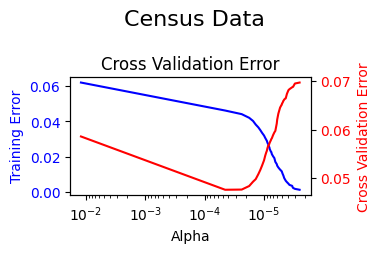
\includegraphics[width=2.75in]{figures/Census_Data_decision_tree_cross_validation.png}
\caption{Census Data Cross Validation.  The cross validation error starts to rise as the decision tree starts to over fit.  The best cross validation $\alpha$ value of 0.0000153 had a test accuracy of 95.24\%, which was very close to the actual best testing score of 95.30\%. }
\label{fig:census_data_decision_tree_cross_validation}
\end{figure}

I used the DecisionTreeClassifier algorithm from the sklearn library.  By default, this uses a GINI index to split the data.  It was possible to use an information gain entropy for splitting, but this did not make a meaningful difference in results for the datasets so the GINI index was used.  A key aspect of sklearn is that it only accepts numeric data for features and treats all features as continuous.  Because of this, a feature can appear in multiple nodes within the same path, with different thresholds.  It also means this is a binary tree, with each node having only two edges.  Other decision tree implementations might allow for discreet features, meaning a feature could only appear once in any tree path and the tree might not be binary.  

At first I thought this would make the tree more complex, but I think there is a reasonable tradeoff.  A tree that always creates a node for all discrete values will always create the maximum amount of nodes but only adds one level of depth to the tree.  The sklearn continous tree may not need to create nodes for every value, but it will end up with greater depth if more than one node needs to be created.  

sklearn also uses a randomizing element, which means that given the same set of data, it may produce different results each run.  In order to produce consistent, repeatable results, the random state setting was set to a fixed value to produce the same results each time.

I used the sklearn Cross Validation module for estimating the best solution without using the test data as described in more detail below.



\begin{figure}[h]
\centering
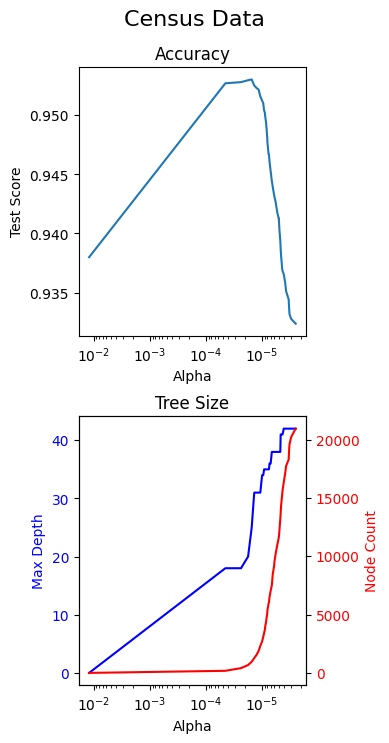
\includegraphics[width=2.75in, height=4in]{figures/Census_Data_decision_tree.png}
\caption{Census Data Decision Tree:  The right side of the upper chart shows overfitting as the pruning is reduced and the number of nodes and tree depth increases.  An unusual aspect is the left side of the chart shows very high accuracy with very few nodes.  This stems from one feature being highly correlated to the labeled output.}
\label{fig:census_data_decision_tree}
\end{figure}

To prune the tree, sklearn uses a minimal cost-complexity setting.  Each node in a tree has an $\alpha$ value which measures the node misclassifications minus leaves misclassifications divided by the number of leaf nodes.  The DecisionTreeClassifier then takes an $\alpha$ minimum setting, pruning all subtrees with a lower $\alpha$.   For both datasets, an accuracy curve was created by fitting the tree with different $\alpha$ values.  

For both data sets, I also performed cross validation to use the training set only to determine the best $\alpha$ parameter, with a 5 fold setting (80\% of training data used for training, 20\% used for validation).  I would then use the test data at different $\alpha$ values to confirm the finding.

For the Census Data, Figure \ref{fig:census_data_decision_tree_cross_validation} shows the use of cross validation to estimate the best solution, in this case setting for $\alpha$, without using the test data.   The best cross validation $\alpha$ value of 0.0000153 had a test accuracy of 95.24\%, which was very close to the actual best testing score of 95.30\%.  Cross Validation provides a powerful tool for evaluation a given training set without reference to test data when available.

The Census Data, shown in Figure \ref{fig:census_data_decision_tree},  mostly shows the expected curve.  Accuracy improves as nodes are added, to a point, then accuracy declines due to over fitting as more nodes are added.  Alpha, the pruning constant, leaves more nodes in the tree as it is decreased.  The Census Data also showed a unique characteristic.  One of its features (Capital Losses), showed a very high correlation with the labeled output, Income above \$50k.  Thus, a one node tree already showed 94\% accuracy.  Figure \ref{fig:census_data_decision_tree} shows this, with the the left side of the chart with few nodes already having a very high accuracy.  


\begin{figure}[h]
\centering
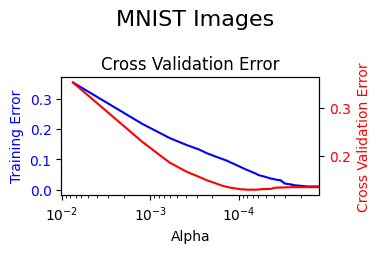
\includegraphics[width=2.75in]{figures/MNIST_Images_decision_tree_cross_validation.png}
\caption{MNIST Images Cross Validation Error:  The chart shows continual reduction in training error, while the Cross Validation error reaches a minimum at an $\alpha$ of 0.0000542 and then starts to rise.  This was very close to the best $\alpha$ found using the testing data. }
\label{fig:MNIST_Images_decision_tree_cross_validation}
\end{figure}

Figure \ref{fig:MNIST_Images_decision_tree_cross_validation}  shows the cross validation error curves for the MNIST image data.  The best cross validation $\alpha$ value of 0.0000762 had a test accuracy of 87.18\%,  while the actual best testing score of 88.54\%.  This was a larger gap than found in the Census data, but still relatively close.

\begin{figure}[h]
\centering
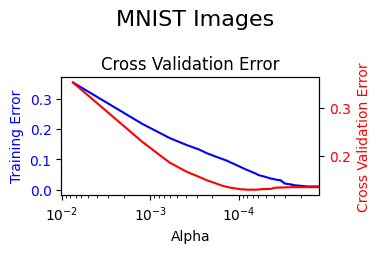
\includegraphics[width=2.75in]{figures/MNIST_Images_decision_tree_cross_validation.png}
\caption{MNIST Images Cross Validation Error:  The chart shows continual reduction in training error, while the Cross Validation error reaches a minimum at an $\alpha$ of 0.0000542 and then starts to rise.  This was very close to the best $\alpha$ found using the testing data. }
\label{fig:MNIST_Images_decision_tree_cross_validation}
\end{figure}

NEED TO FIX

The MNIST image data, shown in Figure \ref{fig:MNIST_Images_decision_tree}, showed a more normal accuracy curve than the Census Data, with accuracy improving dramatically with added nodes until a maximum accuracy was reached, then accuracy declines due to over fitting.  The maximum accuracy achieved was 88.7\%, which was significantly below the census data.  A decision tree is looking at one pixel at a time, 
so small variations in position or size would be very challenging for this algorithm.  I think other classifiers, especially the neural network to better handle image data. 

\section{Neural Networks}
For the neural network, I used PyTorch with two hidden layers, the Adam optimizer and Linear layers.  I then adjusted the size of the layer, the learning rate, and epoch cycles to find the optimal settings.  I used mean squared error loss, which I don't think is a great fit for a binary classification, but had significant trouble getting that type of model to work.  

In just the initial setup for the Census data, I quickly determined I would need to scale the data as the solver would often "blow up" with really large values.  I used the sklearn StandardScaler module, which removes the mean from each feature then applies a sigmoid function to create values from -1 to 1.  This is somewhat suspect for the categorical features, as there is not really a positional relationship, but it was still effective.  I also changed my cross validation process.  I used a 4 folds instead of 5 as I became more worried about the small amount of positive labels.  This also speeded up processing.  In addition, I created my own cross validation process because of my custom neural network. 

\begin{figure}[h]
\centering
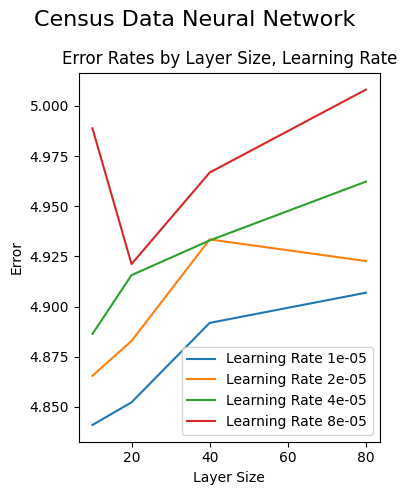
\includegraphics[width=2.5in, height=2.5in]{figures/Census_Data_Neural_Network_Error_Rates_by_Layer_Size__Learning_Rate_census.png}
\caption{Census Data Neural Network:  Built using PyTorch, linear functions and two hidden layers.  The lowest error is clearly shown for the smaller learning rate with the smaller network.   }
\label{fig:census_neural_network_start}
\end{figure}

Figure \ref{fig:census_neural_network_start} clearly shows the preference for the smaller layer size and smaller learning rate, although the differences in absolute accuracy are quite small.  This is a victory still due to the very skewed dataset, with only ~6\% of the data being labeled positively.  The smaller layer size performance is straight out of the class lecture with regard to preferring simpler solutions.  I had expected larger layer sizes to be more effective.  The charts indicates that further exploration at the lower end was worthwhile.

\begin{figure}[h]
\centering
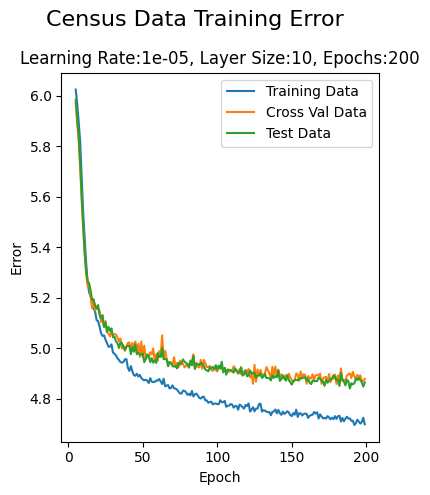
\includegraphics[width=2.5in, height=2.5in]{figures/Census_Data_Training_Error_Learning_Rate_chart_one.png}
\caption{Census Data Neural Network Training Error:  It shows that the cross validation error was very close to the real test data error and a good guide for decision making.  }
\label{fig:census_neural_network_error}
\end{figure}

Figure \ref{fig:census_neural_network_error} shows one of the best performing settings from the initial review.  It shows that the cross validation error was very close to the real test data error and a good guide for decision making.  The chart also doesn't clearly have a movement up of the cross validation error, indicating more epoch training could be beneficial.

\begin{figure}[h]
\centering
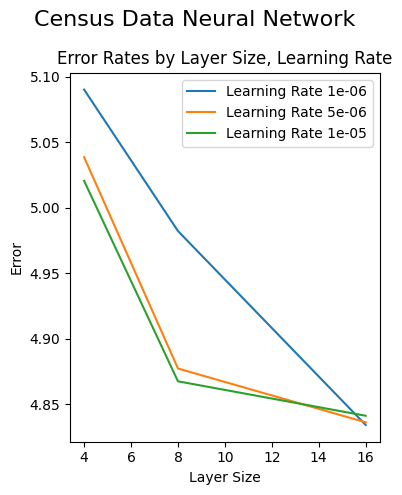
\includegraphics[width=2.5in, height=2.5in]{figures/Census_Data_Neural_Network_Error_Rates_by_Layer_Size__Learning_Rate_census_v2.png}
\caption{Census Data Neural Network:   Lower settings for layer size and learning rate were used in testing.   However, the absolute gains were very, very small, indicating the maximum performance for this dataset.   }
\label{fig:census_neural_network_v2}
\end{figure}

I then tried a new round of testing with lower learning rates, smaller network sizes and longer epoch training.  Those results are shown in Figure \ref{fig:census_neural_network_error}.  The absolute gains over in performance where very, very small, indicating that this was the practical limit of performance.  The best result was with a learning rate of 0.000001, hidden layer size of 16, with the best result coming around 600 epochs of training.  This performed worse than the decision tree. 

For the MNIST data, I created a different neural network topology.  The PyTorch site has many helpful resources and tutorials [3] providing good guidance for one hot encoding.  The MNIST dataset is a very popular one and there are many neural network implementations, but I stuck to refereing to the general PyTorch tutorial.I was able to use this as a skeleton to explore the algorithm and the data. I kept the image data flattened, creating 784 input features.  I then had two hidden layers, the first with 120 nodes, the second with 84 nodes.  For the output, I used one hot encoding on the labels, with one bit for each value between 0 and 9, creating 10 outputs.  To convert the 10 outputs to a single integer, the bit with the highest value is chosen.  I did not initially include any convolutional layers to allow for a more accurate comparison between the decision tree and the neural network.

For this network, I used a different loss function, Cross Entropy Loss, to account for the single selection amongst one of ten output bits.  I also used the SGD optimizer with momentum. 

\begin{figure}[h]
\centering
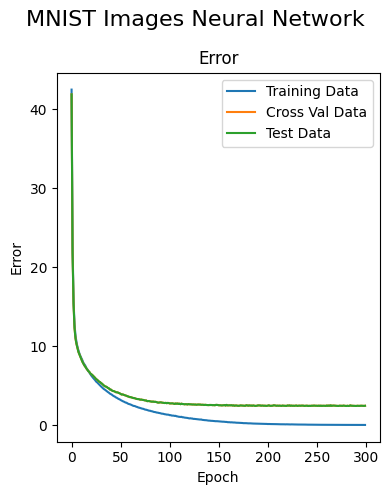
\includegraphics[width=2.5in, height=2.5in]{figures/MNIST_Images_Neural_Network_Error_MNIST.png}
\caption{MNIST Neural Network:  This uses the flattened images and no convolutional networks, with a cross validation using a 4 fold split.  The cross validation error closely tracking the test set error. The best accuracy reached was 97.27\%,  with 275 epoch of training.  }
\label{fig:MNIST_Error_neural_network}
\end{figure}

Figure \ref{fig:MNIST_Error_neural_network} shows the result of the initial review with the flattened images.  Cross validation closely tracks the test accuracy, indicating it is a good tool for decision making.  The training improvement plateaued around 275 epochs of training.  The best accuracy reached here was 97.27\%, which is ~9\% better than the decision tree.  I think this is a result of several things.  From the dataset's standpoint, it is a completely continuous data set, with no discrete values, which is better for the linear layers of the neural network.  It is also a less noisy dataset, with a reasonable outcome expected for each instance.  In contrast, the Census data does not have a necessary relationship, with some instances conflicting with other ones on output labels.  I also think the cross entropy loss function is also much better fit for this classification problem.

A key distinction in the MNIST dataset is that each feature has a spatial relationship to the others, in the form of a 2 dimensional grid.  It is a common practice to use convolutional networks to take advantage of that relationship.  I added two convolutional networks to the beginning of the network.  The first added 10 channels and used a kernel size of 5.  This means that for each 5 X 5 grid, a 5 X 5 filter is applied that multiplies each grid by the filter number, then sums the results.  This is moved over all parts of the image and allows for spatial features to be highlighted.  There is a different filter for each channel, with the different filters enhancing aspects of the grid, like edge detection.  Without padding the image, this will result in an output that has 4 less on each dimension, reducing the 28 X 28 grid to 24 X 24.   There is then a pooling layer that takes each 2 X 2 grid and choses the max value.  This reduces teach dimension by 2, changing the 24 X 24 grid to 12 X 12.  Another convolutional layer was added with 20 channels, leading to an output of 20 X 4 X 4.  This was then connected to the previous network.

\begin{figure}[h]
\centering
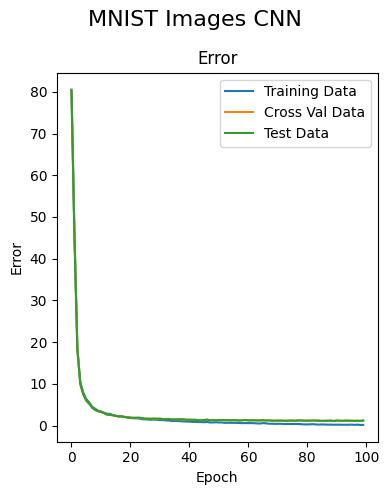
\includegraphics[width=2.5in, height=2.5in]{figures/MNIST_Images_CNN_Error_MNIST.png}
\caption{MNIST Convolutional Neural Network:  This network used two convolutional layers, creating much better performance.  It reached the the same accuracy as the non CNN network in ~13 epochs, which took 275 epochs.  The overfitting is just starting to be seen around 100 epochs. }
\label{fig:MNIST_Error_MNIST_cnn}
\end{figure}

The results were much better using the convolutional networks.  Figure \ref{fig:MNIST_Error_MNIST_cnn} shows the great increase in performance, with it reaching the the same accuracy of the non CNN network in 13 epochs vs 275 epochs.  However, the training time was much greater, with the CNN layers requiring significant processing time. The maximum accuracy also improved by ~1.5\% to 98.89\%.  This improvement in accuracy is significant as the the last few percentage points in accuracy make the difference in many real world settings between success and failure. 

Overall, the CNN layers represent use of domain knowledge about image data and demonstrate the flexible power of neural networks.  

\section{Boosting}

\begin{figure}[h]
\centering
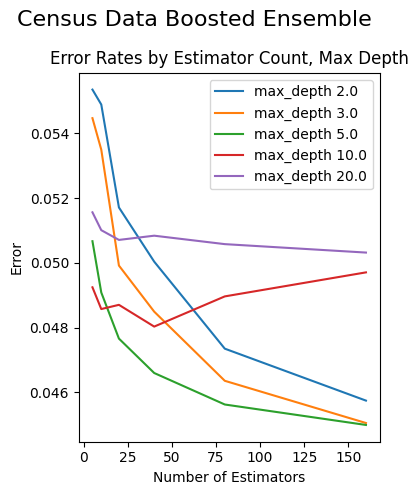
\includegraphics[width=2.5in, height=2.5in]{figures/Census_Data_Boosting_Estimator_Count_by_Max_Depth_boosting_1.png}
\caption{Boosting Census Data Max Depth:  This shows error rates with different number of estimators and different Max Depths of the estimators.  Max features was set to 3. }
\label{fig:boosting_census_1}
\end{figure}

\begin{figure}[h]
\centering
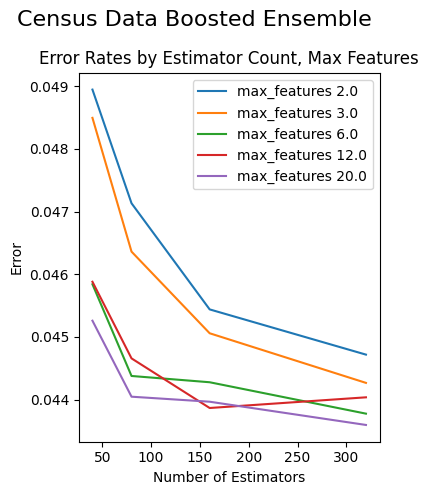
\includegraphics[width=2.5in, height=2.5in]{figures/Census_Data_Boosting_Estimator_Count_by_Max_Depth_boosting_2.png}
\caption{Boosting Census Data Max Features:  This shows error rates with different number of estimators vs the maximum number of features for each tree. Maximum depth was set to 3  }
\label{fig:boosting_census_2}
\end{figure}

\begin{figure}[h]
\centering
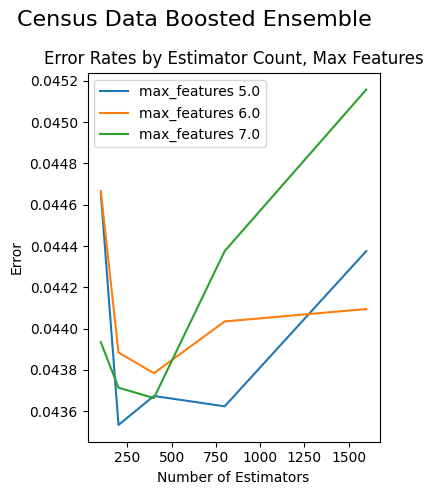
\includegraphics[width=2.5in, height=2.5in]{figures/Census_Data_Boosting_Estimator_Count_by_Max_Depth_boosting_3.png}
\caption{Boosting Census Data Max Features:  This shows over fitting after 800 estimator trees.  Maximum depth was set to 3  }
\label{fig:boosting_census_3}
\end{figure}

\begin{figure}[h]
\centering
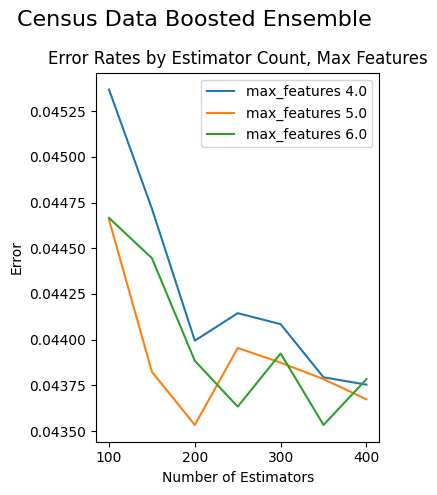
\includegraphics[width=2.5in, height=2.25in]{figures/Census_Data_Boosting_Estimator_Count_by_Max_Depth_boosting_4.png}
\caption{Boosting Census Data Final Review:  Max Features of 5 at 200 estimators is found to be the best solution, achieving  95.65\% }
\label{fig:boosting_census_4}
\end{figure}

I chose to use the sklearn GradientBoostingClassifier for boosting.  I set the classifiers loss setting to "exponential" so that is reverts to the ADABoost algorithm. Without this setting, the classifier uses a more complex loss function and it does a gradient descent.  I chose the ADABoost because it was closer to the algorithm discussed in class.

Two of the key considerations when working with ensemble boosting is how many learners to use and how "weak" the learners are.  The Max Depth setting determines what the maximum depth of each of the estimator trees is.  By making this small, the learners become less accurate, but also less prone to overfitting. Figure \ref{fig:boosting_census_1} shows how increasing depth up to 5 improves performance, but at depths over 10 performance decreases and becomes erratic.  The change at higher levels is somewhat counter intuitive, as the individual learners are more accurate, but is likely due to the fact that the more accurate learners are overfitting.  Figure \ref{fig:boosting_census_1} also shows how adding estimators improves performance, although with diminishing returns.  

I then focused on reviewing the number of features setting.  The classifier will consider a maximum number of features chosen at random for each tree.  Generally, lower numbers make the learners less accurate, high numbers may be better initially but allow for some overfitting. Figure \ref{fig:boosting_census_2}  shows that while considering up to 20 features is the best, 6 features is very close.

Figure \ref{fig:boosting_census_3}  shows overfitting after 400 - 800 estimators, leading to a final review with lower feature counts focused on 80-320 estimators.

Figure \ref{fig:boosting_census_4}  shows maximum features of 5 with 200 estimators is found to be the best solution, achieving  95.65\%.  This is better than the 95.30\% achieved with the decision tree, showing the power of using relatively weak learners in a thoughtful ensemble.

\begin{figure}[h]
\centering
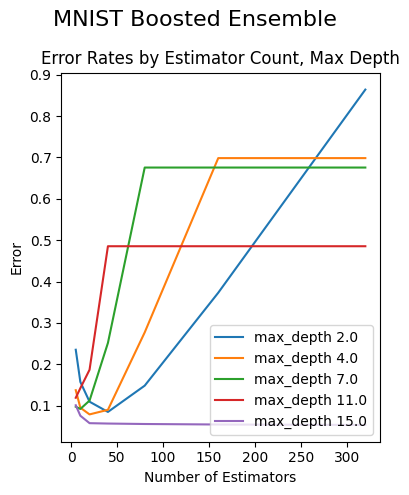
\includegraphics[width=2.5in, height=2.25in]{figures/MNIST_Boosted_Ensemble_boosting_1.png}
\caption{MNIST Data Max Depth:  The chart shows overfitting occuring with relatively few estimators.  Maximum features was set to 28.  }
\label{fig:boosting_mnist_1}
\end{figure}

For the MNIST data, I reviewed the estimator count vs max depth to begin with.  I set the maximum features to 28, the square root of the features, which is a commonly used starting point.

Figure \ref{fig:boosting_mnist_1}  shows overfitting with relatively few estimators.  An interesting point is that the over fitting then reaches a plateau, which may be from the interplay between maximum features and maximum depth.  It is also a bit hard to make sense of the max depth, as the best performing are the low of 2,4, and high of 15. 

\begin{figure}[h]
\centering
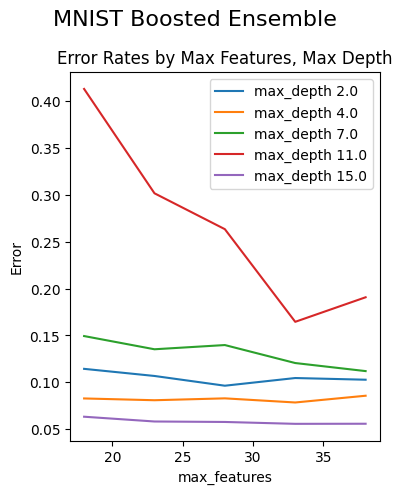
\includegraphics[width=2.5in, height=2.25in]{figures/MNIST_Boosted_Ensemble_boosting_2.png}
\caption{MNIST Data Max Feature vs Max Depth:  This shows that the best performing max depth is 15, then 4, then 2.  It is odd that the high and low maximum depths perform better. The number of estimators was 25.  }
\label{fig:boosting_mnist_2}
\end{figure}

More review was then performed using a fixed number of estimators, 25. Figure \ref{fig:boosting_mnist_2} shows the result, with the best results being a max depth of 15, with more features generally performing better.

\begin{figure}[h]
\centering
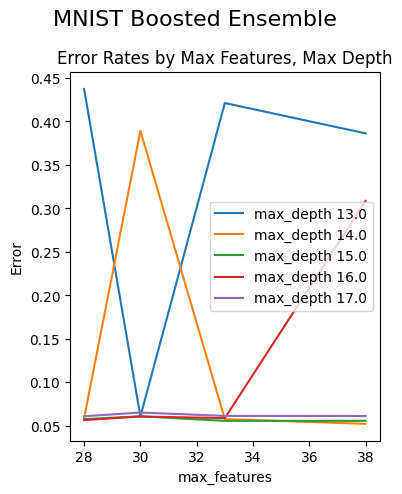
\includegraphics[width=2.25in, height=2.5in]{figures/MNIST_Boosted_Ensemble_boosting_3.png}
\caption{MNIST Data Max Feature vs Max Depth:  The number of estimators was 25.  }
\label{fig:boosting_mnist_3}
\end{figure}

The final review, seen in Figure \ref{fig:boosting_mnist_3}, shows the best performance with a max depth of 14 and max features of 38.  This achieved accuracy of 94.44\%, which is significantly better than the decision tree, but not as good as the neural network.  This makes sense, as the boosted ensemble is better able to deal with the large number of features, but still doesn't take optimum advantage of the spatial relationships in image files.


\section{Support Vector Machines}

I chose to use SVC from the sklearn library.  The key area for review was the use of different kernels.  For both datasets, the following kernels were tested: Linear, Polynomial with 3rd degree, Radial Bias Function, and Sigmoid.

\begin{figure}[h]
\centering
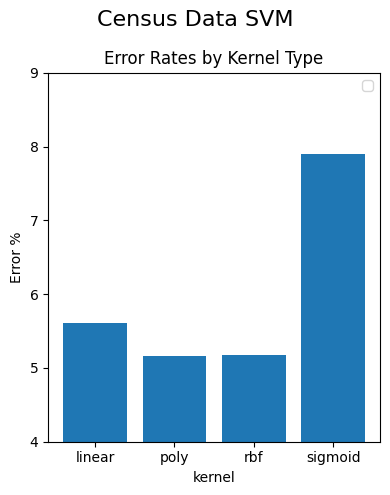
\includegraphics[width=2.5in, height=2.5in]{figures/Census_Data_SVM_svm_1.png}
\caption{Census Data SVM Classifier:  Error rate by different kernel types.  }
\label{fig:svm_census_1}
\end{figure}

\begin{figure}[h]
\centering
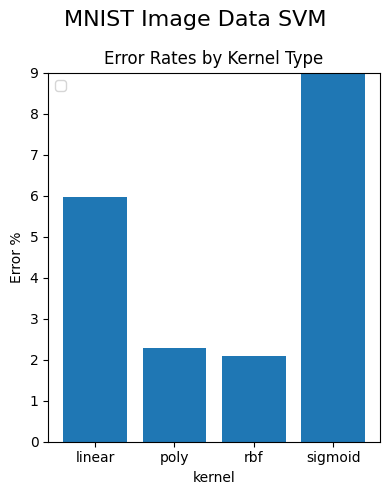
\includegraphics[width=2.5in, height=2.5in]{figures/MNIST_Image_Data_SVM_svm_1.png}
\caption{MNIST Images SVM Classfier:  Error rate by different kernel types.  }
\label{fig:svm_mnist_1}
\end{figure}

The Census Data review is seen in Figure \ref{fig:svm_census_1}.  This shows that the Polynomial (3rd degree) and Radial Bias kernels performed the best.  The slight winner was Polynomial, with a test accuracy of  94.83\%.  A key thing to note is that the SVC solver took the longest time to solve of any of the different algorithms.  The dataset size, with almost 200,000 training instances is a significant challenge to this solution type.

\section{K-Nearest Neighbors}
I used the sklearn KNeighborsClassifier for the K-Nearest Neighbors classifier, with key settings for review were the appropriate number of neighbors, the distance method and potentially weighting based on distance.  One thing to note is that K-Nearest Neighbors is a lazy learner, which in this application means that the fit function, which is used in the classifier models, is very fast, mostly just loading the training data.  It is on the predict function that the learner takes its time.


\begin{figure}[h]
\centering
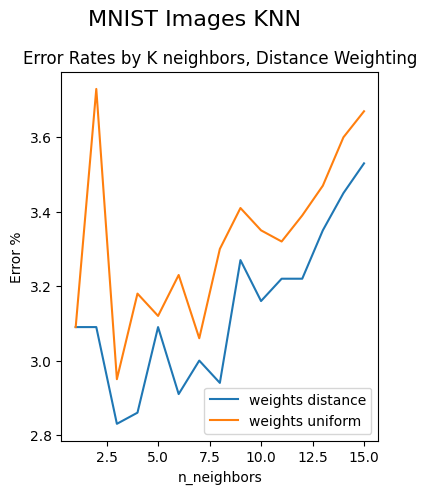
\includegraphics[width=2.5in, height=2.5in]{figures/MNIST_Images_KNN_knn_1.png}
\caption{MNIST Images KNN:  Error rate by different settings of K and different weightings of neighbors by distance.  Uniform means all neighbors are weighted the same, distance means neighbors are weighted by the inverse of distance.  }
\label{fig:mnist_knn_1}
\end{figure}

Figure \ref{fig:mnist_knn_1} shows the MNIST KNN classifier.  The best value of K is 3 with neighbors weighted by inverse of distance.  Overall, this performs very well, with an overall accuracy of 97.17\%, the second best of all algorithms.  The strong performance for the MNIST images is driven by several things.  The algorithm effectively uses all the feature data, because all are calculated in the distance metric.  With all features being continuous and originally on the same scale, the distance metric is an effective way to compare all features.  The intuition is that similar numbers will be closer for each pixel \ feature than dissimilar ones.  For example, two zeros may not line up perfectly, but they will have closer pixels that a one and a zero.  Weighting neighbors by their distance enhances this, making less likely neighbors less impactful.   The small K also makes sense because numbers may be shifted in the image. For example, two images of a 1 with one shifted to the left would have a big distance, as almost no pixels are a match.  In this case, a large K would allow other images with a big distance to be selected, like a 0 which does cross over a 1 in several places.  A small K restricts this selection to more likely true matches.

The weakness for this algorithm is that it really isn't generalizing, but is very dependent on its training set having similar examples to the test set.



\section{References}
\begin{tabular}{l p{2.75in}}
\\
1 & Census Income (KDD). url: https://archive-beta.ics.uci.edu/ml/datasets/census+income+kdd.
\\
2 & The MNIST Database of Handwritten Digits. url: http://yann.lecun.com/exdb/mnist/.
\\
3 & Pytorch Tutorial on Training a Classifier. url: https://pytorch.org/tutorials/beginner/blitz/cifar10\_tutorial.html.
\end{tabular}
\end{document}
